\section*{4/8}
  \subsection*{Conditioning}
    \underline{Conditional probability}: $P(E|F) = \frac{P(E\bigcap F)}{P(F)}$\\
    \underline{Conditional pmf}: $p_{X|Y}(x|y) = \frac{p(x,y)}{p_Y(y)} = P(X=x|Y=y)$\\
    \underline{Conditional density}: $f_{X|Y}(x|y) = \frac{f(x,y)}{f_Y(y)}$\\

    \noindent\underline{Example}: $X,Y$ are independent Poisson: $EX= \lambda_1$, 
      $EY = \lambda_2$. Conditional probability mass function of $X$ given
      $X+Y = n$.\\
      \begin{eqnarray*}
        P(X = k| X+Y = N) & = & \frac{P(X = k, X+Y = n)}{P(X+Y = n)}\\
        & = & \frac{P(X= k)P(Y = n-k)}{\frac{(\lambda_1 + \lambda_2)^n}{n!}
          e^{-(\lambda_1 + \lambda_2)}}\\
        & = & \frac{\frac{\lambda_1^k}{k!} e^{-\lambda_1} 
              \cdot \frac{\lambda_2^{n-k}}{(n-k)!} e^{-\lambda_2}}
          {\frac{(\lambda_1 + \lambda_2)^n}{n!} e^{-(\lambda_1 + \lambda_2)}}\\
        & = & \binom{n}{k} \left(\frac{\lambda_1}{\lambda_1 + \lambda_2}\right)^k
          \left(\frac{\lambda_2}{\lambda_1 + \lambda_2}\right)^{n-k}\\
      \end{eqnarray*}
      We have $Binomial(n, \frac{\lambda_1}{\lambda_1 + \lambda_2})$.\\\\
    \underline{Example}: $T_1, T_2$ are two independent exponential($\lambda$).\\
    Let $S_1 = T_1$, $S_2 = T_1 + T_2$.\\
    Compute $f_{S_1|S_2}(s_1 | s_2)$ or $\frac{f(s_1, s_2)}{f_{S_2}(s_2)}$.\\
    First,
    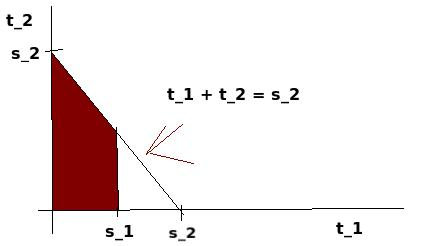
\includegraphics{4_8.jpeg}
    \begin{eqnarray*}
      P(S_1 \le s_1, S_2 \le s_2) 
        & = & P(T_1 \le S_1 , T_1 + T_2 \le S_2)\\
        & = & \int_0^{s_1} dt_1 \int_0^{s_2 - t_1} dt_2 f_{T_1, T_2}(t_1, t_2)\\
      f(s_1, s_2) 
        & = & \frac{\sigma}{\sigma s_2}\int_0^{s_2 - s_1} dt_2 f_{T_1, T_2}(s_1, t_2)\\
        & = & f_{T_1, T_2}(s_1, s_2 - s_1)\\
        & = & f_{T_1}(s_1)f_{T_2}(s_2 - s_1)\\
        & = & \lambda e^{-\lambda s_1} \lambda e^{-\lambda (s_2 - s_1)}\\
        & = & \lambda^2 e^{-\lambda s_2}
    \end{eqnarray*}
    Therefore,
    $$
      f(s_1, s_2) = 
        \begin{cases}
          \lambda^2 e^{-\lambda s_2} & \text{if } 0 \le s_1 \le s_2\\
          0 & \text{otherwise}
        \end{cases}
    $$
    $f_{s_2}(s) = \lambda^2 s_2 e^{-\lambda s_2}$ for $s_2 \ge 0$.\\
    Therefore,
    $$
      f_{S_1| S_2}(s_1 | s_2) = \frac{\lambda^2 e^{-\lambda s_2}}{\lambda^2 s_2 e^{-\lambda s_2}}
         = \frac{1}{s_2}
    $$
    give that $0 \le s_1 \le s_2$ and 0 otherwise.\\
    Therefore, given that if we know when the second bulb fails, the first 
    bulb can fails follow the uniform distribution between $0$ and $s_2$.

  \subsection*{Computing expectataions and probability by conditioning}
    \underline{Example}: Roll a die. Assume the number rolled is $N$.
      Then, continue rolling until you either match or exceed $N$.
      What is the expected number of additional rolls?\\
      This is geometric if we know $N$, so let's condition on the
      value of $N$.\\
      Let $X$ be the number of additional rolls.\\

      \begin{eqnarray*}
        E(X|N = n)
          & = & \frac{6}{7-n}\\
        E(X) 
          & = & \sum_{n = 1}^6 E(X|N = n) P(N = n)\\
          & = & \frac{1}{6}\sum_{n=1}^6 \frac{6}{7-n}\\
          & = & \sum_{n=1}^6 \frac{1}{7-n}\\
          & = & 1 + \frac{1}{2} + \frac{1}{3} + \ldots + \frac{1}{6}
      \end{eqnarray*}
    \underline{Example}: the number $N$ customers entering a store on a given 
      day is $Poisson(\lambda)$. Each of them buys something independent with
      probability $p$.\\
      Compute the probability that $k$ people buy something.\\
